\documentclass[landscape]{foils}
\usepackage[pdftex]{color}
\usepackage[pdftex]{graphicx}
\usepackage{eso-pic}
\usepackage[top=2cm, bottom=2cm, outer=0cm, inner=0cm]{geometry}\usepackage{listings}
\usepackage{amsmath}
\usepackage{hyperref}


\DeclareMathOperator{\sign}{sign}

% colors
\definecolor{DarkRed}{rgb}{0.5,0.0,0.0}
\definecolor{DarkBlue}{rgb}{0.0,0.0,0.35}
\definecolor{DarkGreen}{rgb}{0.0,0.6,0.00}
\definecolor{Orange}{rgb}{0.70,0.30,0.0}
\definecolor{Magenta}{rgb}{0.8,0.0,0.8}
\definecolor{DarkGray}{rgb}{0.3,0.3,0.3}
\def\red{\color{red}} 
\def\darkred{\color{DarkRed}} 
\def\blue{\color{DarkBlue}} 
\def\green{\color{DarkGreen}} 
\def\orange{\color{Orange}}
\def\magenta{\color{Magenta}}
\def\black{\color{black}}
\def\gray{\color{DarkGray}}

% sizes, footer and headers
\textwidth = 26truecm
\textheight = 18truecm
\topmargin =-2 cm
\oddsidemargin -1.5cm
\rightfooter{}
\MyLogo{\darkred {\bf QE-2019}: Summer School on Advanced Materials
  and Molecular Modelling}
%
\def\indent{\hspace*{1cm}}
\def\prompt{\texttt{\$~}}
\def\exec#1{\indent\prompt\code{#1}}
\def\codeline#1{\indent\code{#1}}
\parindent 0pt

% alias for slides header
\def\Head#1{\foilhead{\red #1 \vskip -1cm} \medskip\hrule\medskip}
\def\head#1{\foilhead{\red #1 \vskip -1cm}}

% aliases for codes, files, namelists, etc.
\def\codecolor{\green}
\def\cardcolor{\orange}
\def\code#1{\texttt{\codecolor #1}}
\def\prog#1{\texttt{\red #1}}
\def\var#1{\texttt{\red #1}}
\def\file#1{\texttt{\green #1}}
\def\cmd#1{\texttt{\green #1}}
\def\nml#1{\texttt{\magenta #1}}
\def\card#1{\texttt{\cardcolor #1}}
\def\flag#1{\texttt{\green #1}}

% aliases for math
\def\vr{\ensuremath{\bm{r}}}
\def\vR{\ensuremath{\bm{R}}}
\def\vk{\ensuremath{\bm{k}}}
\def\vtau{\ensuremath{\bm{\tau}}}


\begin{document}
\AddToShipoutPictureBG*{
\includegraphics[width=\paperwidth,height=\paperheight]{figs/qe2021-background-4x3.png}}

\blue
~\\
\vspace*{4cm}
\MyLogo{~}
\vspace{5em}
\begin{center}
  {\burgundy\LARGE\bf QE-2021: Hands-on session -- Day-3}\\[2em]
  {\burgundy\LARGE (Structural relaxations + NEB; PWTK)}
  ~\\[1.5em]
    %\large Ari Paavo Seitsonen, Anton Kokalj, Pietro Delugas,\\
  %Matic Poberžnik, Mandana Safari, Unmesh Mondal, Tao Jiang
\end{center}

%%%%%%%%%%%%%%%%%%%%%%%%%%%%%%%%%%%%%%%%%%%%%%%%%%%%%%%%%%%%% 
\Head{QE-2021: Hands-on session -- Day-3}
\MyLogo{\burgundy {\bf QE-2021}: MaX School on Advanced Materials and Molecular Modelling}
\rightheader{\hspace{-0.8cm}
\includegraphics[width=4.5cm]{figs/QE.png}}
Topics of Day-3 hands-on session:
\begin{itemize}
\item Structural optimizations:
  \begin{itemize}
  \item relaxations -- atomic positions only (\file{example1.relax})
  \item variable-cell relaxations (\file{example2.vc-relax})
  \end{itemize}
\item NEB method: saddle points of elementary chemical
  reactions (\file{example3.neb/})
\item Automating the workflow with PWTK
  (\file{example4.pwtk})\\
\end{itemize}

%\vspace{-0.5em}
To get the latest version of the exercises, move to \file{Day-3/} directory and execute:\\[0.5em]
\exec{git pull}

%%%%%%%%%%%%%%%%%%%%%%%%%%%%%%%%%%%%%%%%%%%%%%%%%%%%%%%%%%%%%
\head{How to run calculations remotely on the ``hpc'' HPC cluster}
\rightheader{}

Several utility commands have been implemented specially for the
QE-2021 school to aid at submitting jobs to HPC cluster(s). These are:
{\small
\begin{itemize}
\item \cmd{\bf remote\_mpirun} -- this is like \cmd{mpirun}, but it
  automatically submits the calculation to a queuing system on the
  ``hpc'' HPC system. For example, a \prog{pw.x} calculation can be
  submitted
  as:\\[0.5em]
  \exec{remote\_mpirun pw.x -inp pw.file.in}\\[0.5em]
  where \file{pw.file.in} is the name of the \prog{pw.x} input
  file. {\bf BEWARE:} stdin/stdout redirection does not work for
  \cmd{remote\_mpirun}, hence you must use \flag{-inp} option (i.e.,
  do note use ``\cmd{<}'' redirection operator). You do not need to
  specify the number of processors, because the default is set to
  \flag{-np~8}.
  \vspace{0.5em}
\item \cmd{\bf remote\_pwtk} -- this automatically submits the PWTK
  script to queuing system on the ``hpc'' HPC system. Example:\\[0.5em]
  \exec{remote\_pwtk script.pwtk}\\[0.5em]
  where \file{script.pwtk} is the name of the PWTK script.
\vspace{0.5em}
\item \cmd{\bf remote\_sbatch} -- automatically submits the Unix-shell
  script to queuing system on the ``hpc''  HPC system. Example:\\[0.5em]
  \exec{remote\_sbatch script.sh}\\[0.5em]
  where \file{script.sh} is the name of the Unix-shell script.

\clearpage
\item \cmd{\bf hpc} -- this makes \cmd{ssh} to ``hpc'' HPC login node,
  such that the user will be located in the same directory as used
  locally \vspace{0.5em}
\item \cmd{\bf rsync\_to\_hpc} -- copies specified files to the
  ``hpc'' cluster to the same directory as is currently
  used locally. Example:\\[0.5em]
  \exec{rsync\_to\_hpc *.in}\\[0.5em]
  This will copy all \file{*.in} files from local directory to the
  same directory on the ``hpc'' cluster.  \vspace{0.5em}
\item \cmd{\bf rsync\_from\_hpc} -- download the specified file from
  the ``hpc'' cluster from the same directory as is
  currently used locally. Example:\\[0.5em]
  \exec{rsync\_from\_hpc *.out}\\[0.5em]
  This will copy all \file{*.out} files from the ``hpc'' cluster.
\end{itemize}
}
%%%%%%%%%%%%%%%%%%%%%%%%%%%%%%%%%%%%%%%%%%%%%%%%%%%%%%%%%%%%%
\head{1. How to perform structural optimization: graphane}
\rightheader{}
\rightfooter{Example: \file{Day-3/example1.relax}}

\parbox{17cm}{
  \begin{itemize}
  \item Move to \file{Day-3/example1.relax/} directory.\\[0.5em]
    Graphane is like graphene, with an H atom bound to each C atom in
    {\em trans} configuration. You need to optimize atomic positions,
    i.e., find the minimum-energy structure (zero forces).
  \end{itemize}
} \hskip 1cm
\parbox{8cm}{ 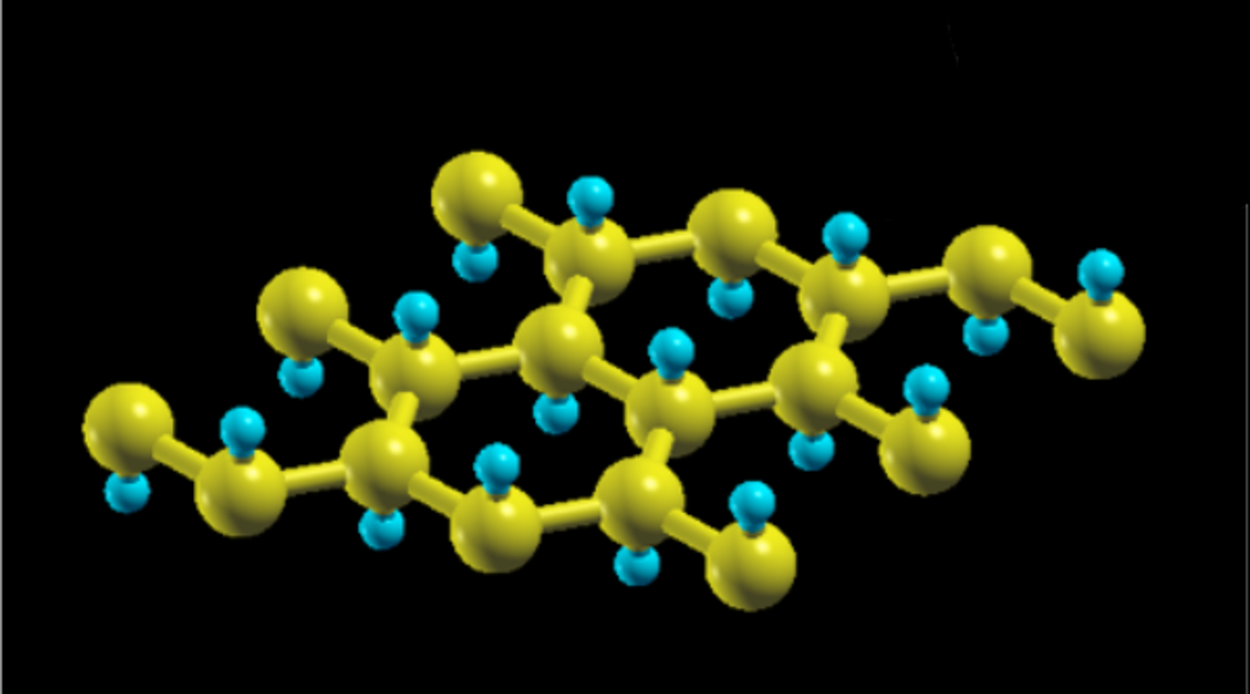
\includegraphics[width=8cm]{figs/graphane.pdf}}

\begin{itemize}
\item File \file{pw.graphane.relax.in} is a modified version of\\
  \file{pw.graphene1x1.scf.in} with:
  \begin{itemize}
  \item \var{calculation='relax'} for structural optimization and a
    new namelist \nml{\&IONS} with variable \var{upscale=100.0}
  \item \var{ntyp=2} (2 types of atoms), \var{nat=4}
    (4 atoms in the cell)
  \item \card{ATOMIC\_SPECIES} card with 2 species of atoms and
    pseudopotentials
  \item \card{ATOMIC\_POSITION} card with 4 initial positions
    (C--H distance $\sim 1$~\AA)
  \end{itemize}
\end{itemize}

%%%%%%%%%%%%%%%%%%%%%%%%%%%%%%%%%%%%%%%%%%%%%%%%%%%%%%%%%%%%% 
\head{1. How to perform structural optimization: graphane (II)}
\begin{itemize}
\item Run the structural optimization, i.e.:\\[0.5em]
  \exec{pw.x < pw.graphane.relax.in > pw.graphane.relax.out \&}
\item When calculation finishes, analyze the output: it consists of
   several SCF steps, followed by calculation of forces and generation
   of new atomic positions.
\item To visualize the evolution of the structure during structural
   optimization, execute:\\[1em]
   \exec{xcrysden --pwo pw.graphane.relax.out}
\end{itemize}
\parbox{15cm}{Relaxed structure of graphane exhibits ``buckling''.}
\hskip 0.5cm \parbox{8cm}{
  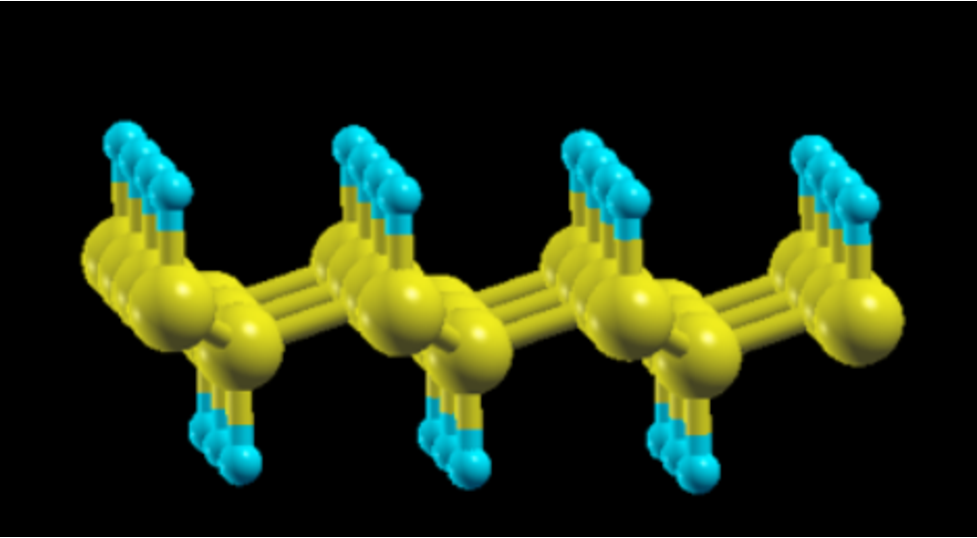
\includegraphics[width=8cm]{figs/graphane2.pdf}
}

%%%%%%%%%%%%%%%%%%%%%%%%%%%%%%%%%%%%%%%%%%%%%%%%%%%%%%%%%%%%% 
\head{1. Supercell and structural optimization: graphene-oxide}

\parbox{15cm}{
  \begin{itemize}
  \item The first stage of graphene oxidation is the formation of an
    epoxy bridge. Let us add an O atom on a $(3\times3)$ supercell of
    graphene
  \end{itemize}
}\hskip 2cm\parbox{7cm}{
  \begin{flushright}
    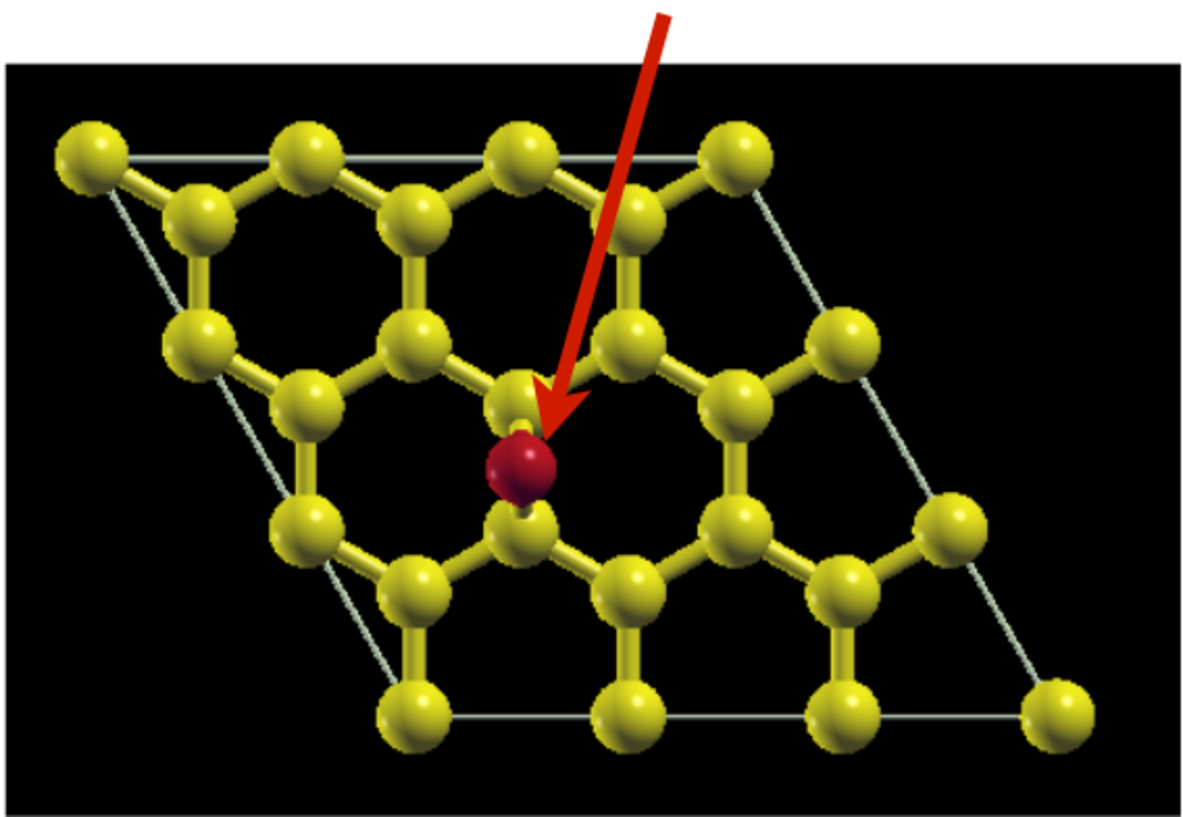
\includegraphics[width=7cm]{figs/graphene3x3-O.pdf}    
  \end{flushright}
}

This example consists of two tasks: (i) build a $(3\times3)$ supercell
of graphene; (ii) add an O atom onto graphene--$(3\times3)$ supercell
structure and run a relaxation calculation.
    
{\bf Step-1:}
\vspace{-1em}
\begin{itemize}
\item The $(3\times3)$ supercell structure of
  graphene is provided in file\\
  \file{pw.graphene3x3.scf.in}, which is a modified version of\\
  \file{pw.graphene1x1.scf.in}. Please
  notice that:
  \begin{itemize}
  \item Lattice parameters $a$ and $b$ are multiplied by 3:
    \var{celldm(1)=13.962}
    \vspace{0.3em}
  \item Lattice parameter $c$ remains the same, hence \var{celldm(3)},
    which equals $c/a$, is divided by 3, hence: \var{celldm(3)=1.0}.
    \vspace{0.3em}
  \item There are 9 times the atoms of the original unit cell, i.e. \var{nat=18}.
    \vspace{0.3em}
  \item Reciprocal lattice vectors in the $xy$ plane are divided by 3
    (look at the output), hence if you want the same k-point grid,
    just use \card{K\_POINTS (automatic)} with \card{3 3 1 0 0 0}
    grid, which is equivalent to \card{9 9 1 0 0 0} k-point grid of
    $(1\times1)$ unit-cell \vspace{0.3em}
  \item Provided that {\burgundy the two k-point grids are equivalent}:
    \begin{itemize}
    \item
      The energy of the supercell $E^{\rm SC} = 9E^{\rm UC}$ almost exactly
      (UC = unit cell)
    \item
      all $\epsilon^{\rm SC}({\bf k}_i)$ are (almost) equal to some
      $\epsilon^{\rm UC}({\bf k}_j)$ if ${\bf k}_j$ refolds into ${\bf k}_i$
    \end{itemize}   
  \end{itemize}
\end{itemize}

{\bf Step-2:}
\vspace{-1em}
\begin{itemize}
\item File \file{pw.graphene3x3-O.relax.in} is a modified version of\\
  \file{pw.graphene3x3.scf.in} with:
  \begin{itemize}  
  \item \var{calculation='relax'} for structural optimization and a new
    namelist \card{\&IONS}
  \item \var{ntyp=2} (2 types of atoms), \var{nat=19}
    (19 atoms in the cell)
  \item \card{ATOMIC\_SPECIES} card with 2 species of atoms and
    pseudopotentials
  \item \card{ATOMIC\_POSITION} card with 19 initial positions
    (C--O distance $\sim 1.5$~\AA)
  \end{itemize}
\item Run the structural optimization and analyze the output
\end{itemize}

%%%%%%%%%%%%%%%%%%%%%%%%%%%%%%%%%%%%%%%%%%%%%%%%%%%%%%%%%%%%% 
\head{2. How to perform variable-cell relaxation: hcp-Zinc}
\rightfooter{Example: \file{Day-3/example2.vc-relax}}
%
Zinc displays an hcp (hexagonal-closed-packed) crystal structure, hence
it has two lattice parameters $a$ and $c$. The unit-cell lattice
vectors are:\\
%
\centerline{$\displaystyle
  {\bf a}_1=(a,0,0), \quad {\bf a_2}=(-{a\over 2},{a\sqrt{3}\over 2},0),
  \quad {\bf a}_3=(0,0,c)$}
%
This lattice can be described as:\\
$\bullet$ \var{ibrav=4}, \var{A=$a$}, \var{C=$c$}, {\em both in \AA,
  not a.u.}, as in file \file{pw.Zn.scf.in}\\
$\bullet$ or \var{ibrav=4}, \var{celldm(1)=$a$}, \var{celldm(3)=$c/a$},
as in the file \file{pw.Zn.vc-relax.in}

For hexagonal lattices one needs to optimize two lattice
parameters. This can be done either {\em manually} or by using the
{\em variable-cell relaxation}. (See also \file{README.md}).
\vspace{-1em}
\begin{enumerate}
\item {\bf Manual way:} to optimize the $a$ and $c$ lattice
  parameters, one need to perform a 2D scan over the two
  parameters. With PWTK this can be achieved with the following
  snippet (full script is available in
  \file{Zn-scan.pwtk}):
  \vspace{-0.5em}
  {\codecolor
\begin{verbatim}
foreach A [seq 2.4 0.1 2.8] {
   foreach C [seq 4.8 0.2 5.6] {
      SYSTEM " A = $A , C = $C"        
      runPW pw.Zn.scf.$A.$C.in
   }
}
\end{verbatim}
  }
\item {\bf Variable-cell relaxation:} This is a more convenient
  option. An example of how to perform variable-cell relaxation is
  provided by the input file \file{pw.Zn.vc-relax.in}. Notice:
  \begin{itemize}
  \item \var{calculation = 'vc-relax'}
  \item \nml{\&IONS} and \nml{\&CELL} namelists are specified after
    the \nml{\&ELECTRONS}
  \end{itemize}
\end{enumerate}
To run the calculation, execute:\\[0.5em]
\exec{pw.x -in pw.Zn.vc-relax.in > pw.Zn.vc-relax.out}

Inspect the output (file: \file{pw.Zn.vc-relax.out}) and notice that:
\vspace{-1em}
\begin{itemize}
  \item several scf steps are performed, forces (zero by symmetry) 
    and stresses computed
    \vspace{-1em}
  \item the energy and the stress decrease as the minimum is approached
    \vspace{-1em}
  \item a final scf step is performed with plane waves computed for
    the final cell
    \vspace{-1em}
  \item the final cell is printed after the last \texttt{CELL\_PARAMETERS}
    card
  \end{itemize}
  Compare optimized parameters estimated from the {\em manual} 2D-scan
  to those obtained from the  {\em variable-cell relaxation}.

%%%%%%%%%%%%%%%%%%%%%%%%%%%%%%%%%%%%%%%%%%%%%%%%%%%%%%%%%%%%% 
\head{2. Variable-cell relaxation (II): molecular crystal of Urea}

While in the preceding example, the forces were zero by symmetry, in
this example (\file{pw.urea.vc-relax.in}) both unit-cell and atomic
positions are optimized by utilizing the {\em variable-cell
  relaxation} (\var{calculation = 'vc-relax'}).  Beware that it is
computationally heavier than the \file{pw.Zn.vc-relax.in} example.
\begin{center}
  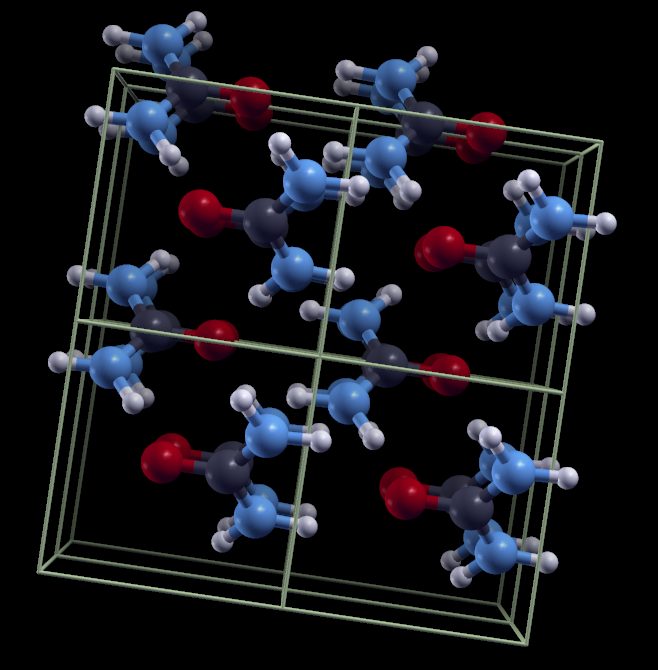
\includegraphics[width=0.4\textwidth]{figs/urea.png}
\end{center}
See the instructions in \file{README.md} for how to run this
calculation remotely.

%%%%%%%%%%%%%%%%%%%%%%%%%%%%%%%%%%%%%%%%%%%%%%%%%%%%%%%%%%%%% 
\head{3. NEB method: saddle points of elementary chemical reactions}
\rightfooter{Example: \file{Day-3/example3.neb}}
%
Saddle points on the {\em Potential Energy Surface (PES)}, which
correspond to {\em Transition States (TS)} of chemical reactions, can
be found by means of the {\em Nudged Elastic Band (NEB)} method.

In the first example we will analyze a simple H transfer reaction:
\begin{center}
{\large $\mathrm{H_2 + H \rightarrow H + H_2}$}
\end{center}
{\bf Example 1a: No intermediate image}

In the NEB method one needs to supply a minimum of two images, the
so-called {\bf first-image} and {\bf last-image}, corresponding to
reactants and products, respectively.

In \file{neb.H2+H.in}, you will see that near the end of the file
\card{FIRST\_IMAGE} and \card{LAST\_IMAGE} are specified. Seven
images are requested (\var{num\_of\_images = 7}) along the
reaction and the \prog{neb.x} code discretizes the path
by means of a linear interpolation.

You can visualize this path with \prog{xcrysden}:

\exec{xcrysden --pwi neb.H2+H.in}

To run the example execute:

\exec{ neb.x -inp neb.H2+H.in > neb.H2+H.out \& }

When the calculation finishes analyze the output
(\file{neb.H2+H.out}). Pay attention to the {\em number of steps} required
to reach convergence and the reaction energy barrier.

\exec{ gnuplot H2+H.gp }

The resulting plot should look something like this.
\begin{figure}
  \centering
    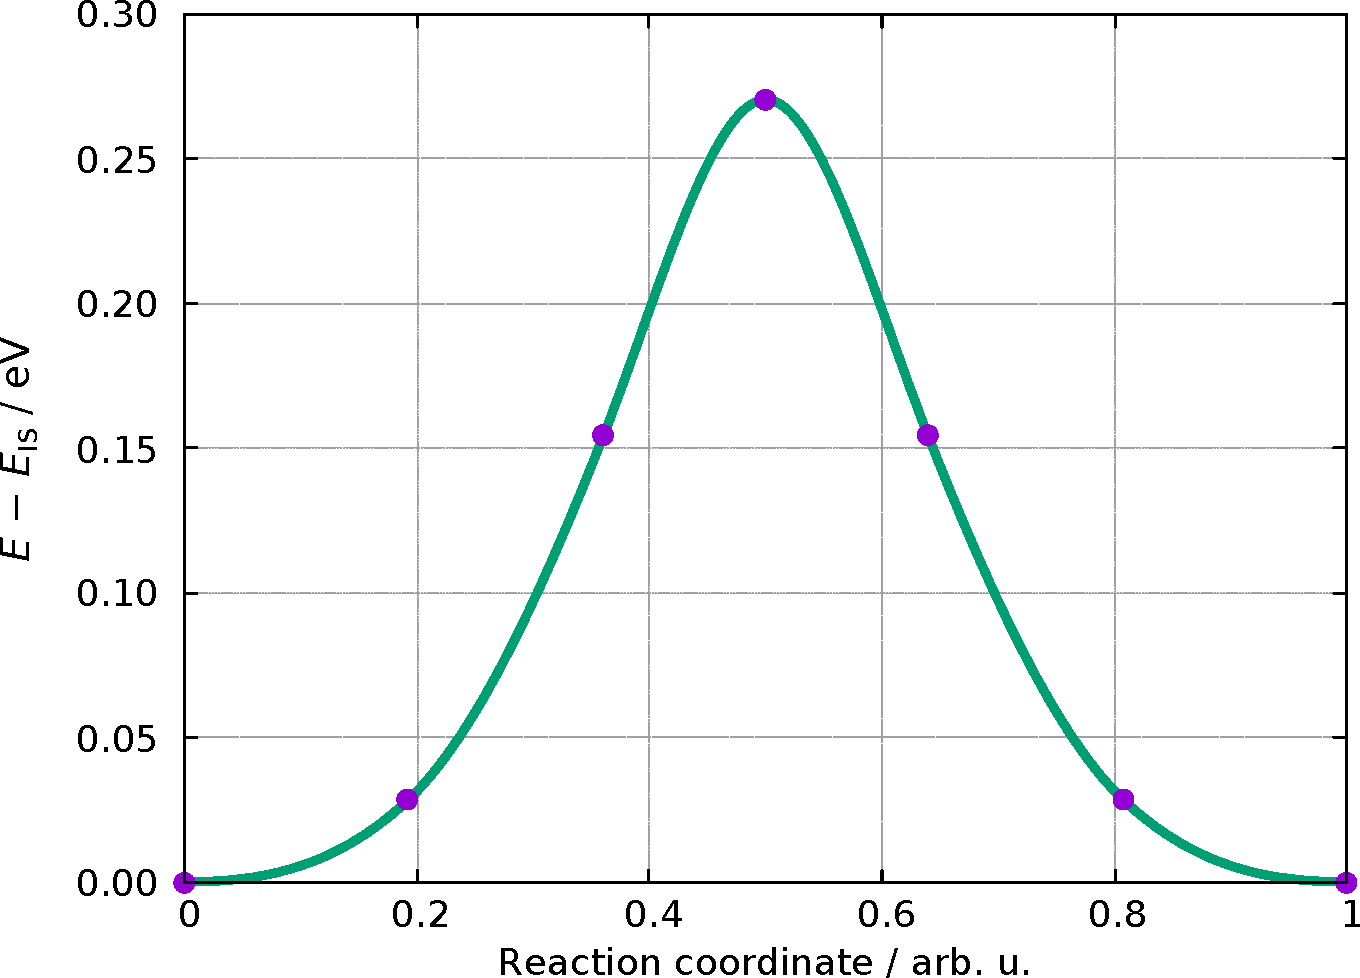
\includegraphics[width=14cm]{figs/H2+H-NEB-path.pdf}
\end{figure}

You can visualize individual points on the reaction path by using \prog{xcrysden}.

Either by typing:

\exec{ xcrysden --xyz H2+H.xyz}

or

\exec{xcrysden --axsf H2+H.axsf}

{\bf Example 1b: NEB with intermediate image}

This example is similar as the previous example, however, chemical
intuition is used now to construct a better initial reaction path. This is
achieved by using the \card{INTERMEDIATE\_IMAGE} card, in which a
rough guess for the transition state is provided. You can visualize
the path by using \prog{xcrysden}:

\exec{ xcrysden --pwi neb.H2+H.w-inter-image.in}

Try to spot the difference between the two examples. Notice that
without the intermediate image, the three atoms are evenly spaced in
the middle of the initial interpolated reaction path, which is not a
good guess of the transition-state. If we use
\card{INTERMEDIATE\_IMAGE} then the three H atoms can be placed closer
together, which is much more similar to the actual transition state and the
NEB calculation does not require as many steps to converge. This is
shown schematically below:

\begin{figure}
  \centering
    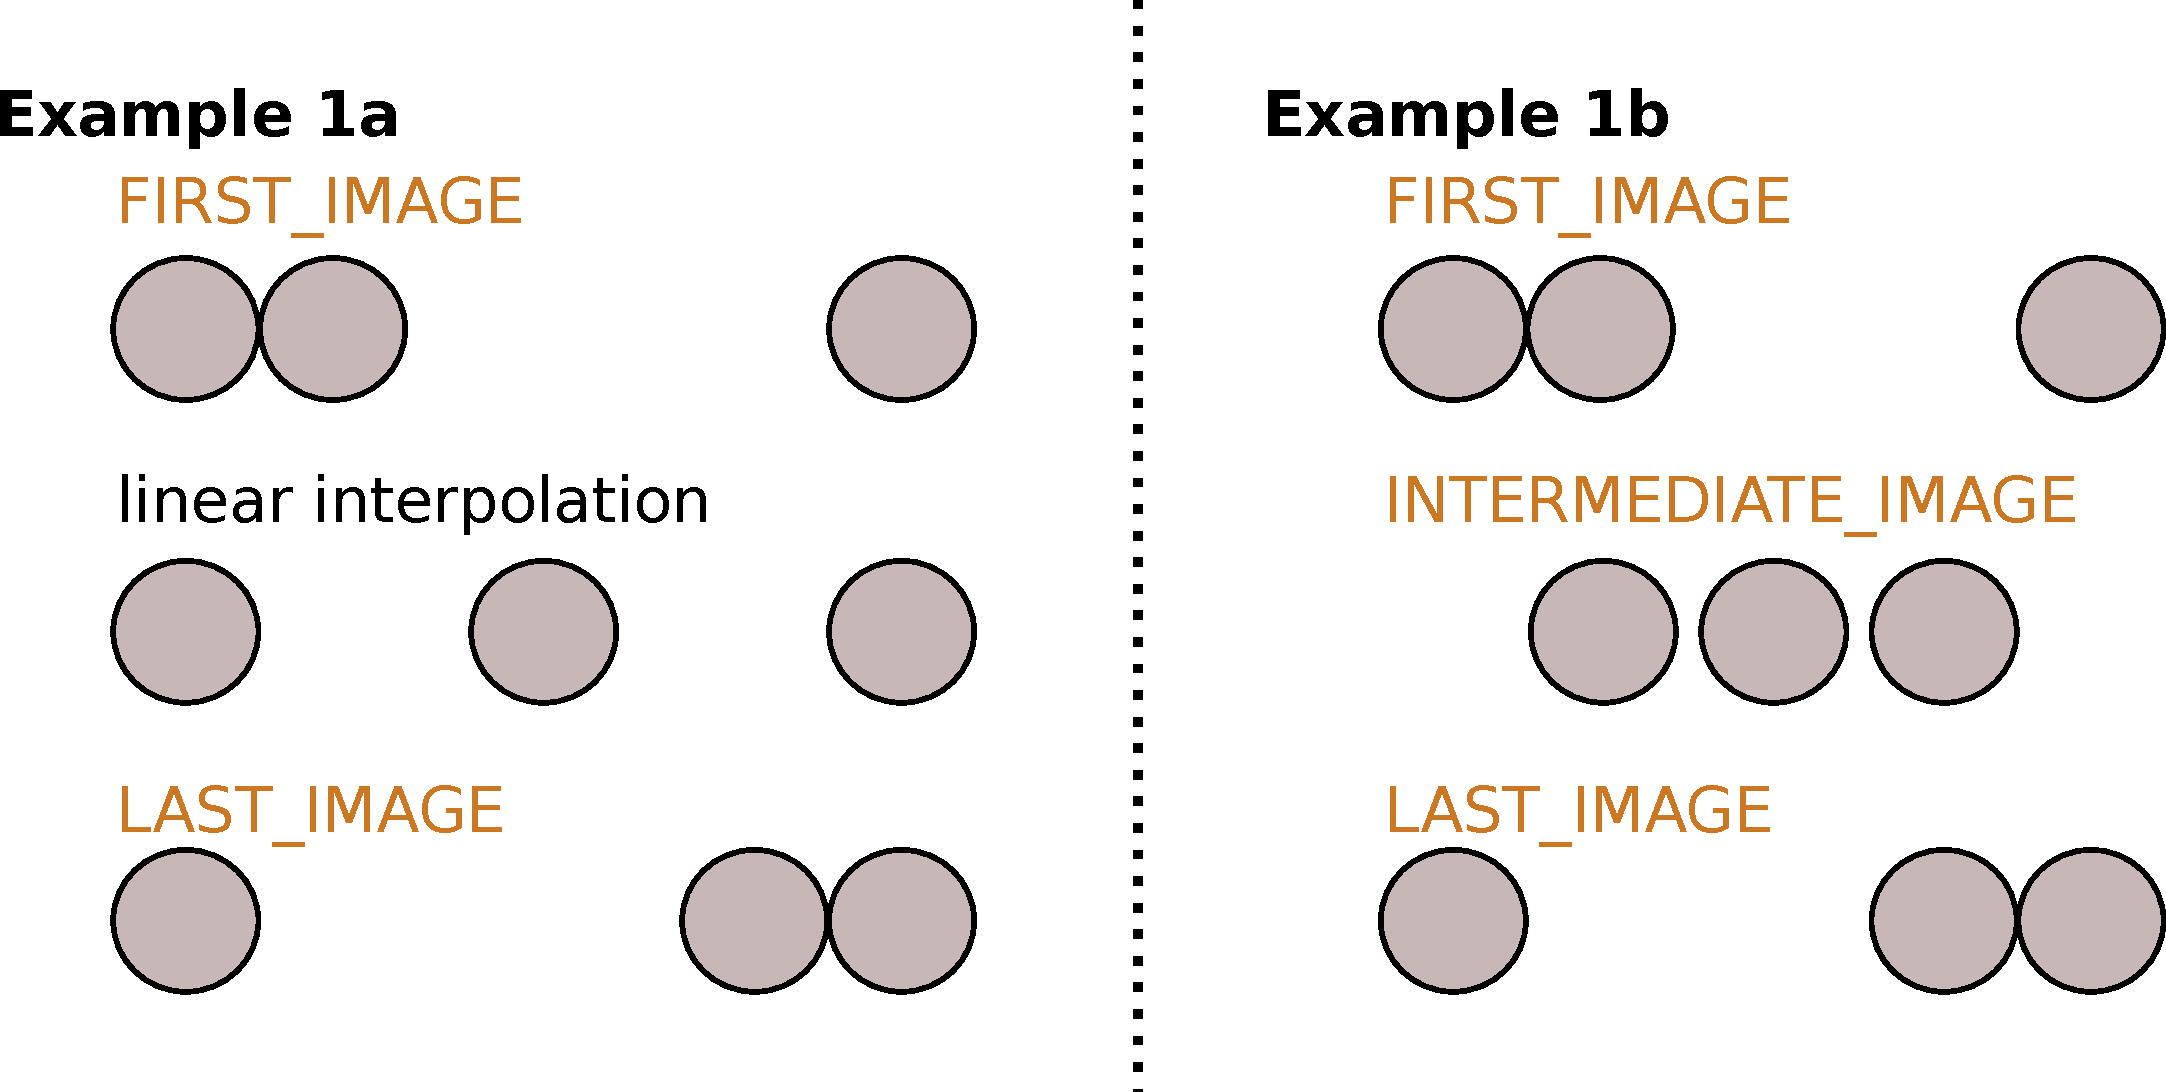
\includegraphics[width=22cm]{figs/neb-w-intermimage.pdf}
\end{figure}

To run this example type:

{\small \exec{ neb.x -inp neb.H2+H.w-inter-image.in > neb.H2+H.w-inter-image.out \& }}

The final reaction barrier should be the same as in the previous
calculation, however convergence should require fewer steps.

{\bf Example 2: A more complex NEB calculation}

In the second example we will study $\mathrm{H_2} $ dissociation on
the Al(100) surface. We will be using \card{INTERMEDIATE\_IMAGE} and
the calculation itself is also divided into two parts, in order to
achieve convergence more quickly.

We will be using climbing-image NEB (CI-NEB), however initially we do
not know which image is the {\em climbing-image} (the one with the
highest energy), because its ID can change from iteration to
iteration, depending on how far from convergence we are.

Thus we will first perform a plain NEB (\var{CI\_scheme = 'no-CI'}) in
order to stabilize the pathway and only once the pathway is stabilized we will
switch on the CI-NEB with \var{CI\_scheme~=~'auto'}. We will use a
PWTK script to manage these two calculations.

{\bf{Steps:}}
\begin{itemize}
\item{Read \file{neb.H2-diss.Al100-2x1-2L.in} and try to understand
    it.
    This file will serve as the main input for the \prog{pwtk} script. Visualize the initial guess by :\\
    \exec{xcrysden --pwi neb.H2-diss.Al100-2x1-2L.in}}
\item{Read the \file{neb.pwtk} script and try to understand it. }
\item{Beware that this example takes about 20--30 min on a
    laptop. Hence, run the calculation remotely, i.e., submit it to
    the HPC cluster, i.e.:\\
    \exec{remote\_pwtk neb.pwtk}}
\item To download the calculated output files, use:\\
  \exec{rsync\_from\_hpc *.out}\\[0.5em]  
  Give the remote computer some time to make the calculation. To
  download other data files that were produced by \prog{neb.x}, use:\\[0.5em]
  \exec{rsync\_from\_hpc .}
\item{Once the calculation converges analyze \file{neb.noCI.out} and
    \file{neb.auto.out} and check the number of steps and the reaction
    energy barrier.
    The reaction energy graph can be plotted by:\\
    \exec{gnuplot H2-diss.Al100-2x1-2L.gp} \\[0.5em]
    and the corresponding path visulized by: \\
    \exec{xcrysden --axsf H2-diss.Al100-2x1-2L.axsf } }
\end{itemize}

\clearpage

\vspace*{1em}
The resulting PES along the reaction coordinate should look like this.

\vspace*{1em}
\begin{figure}
  \centering
    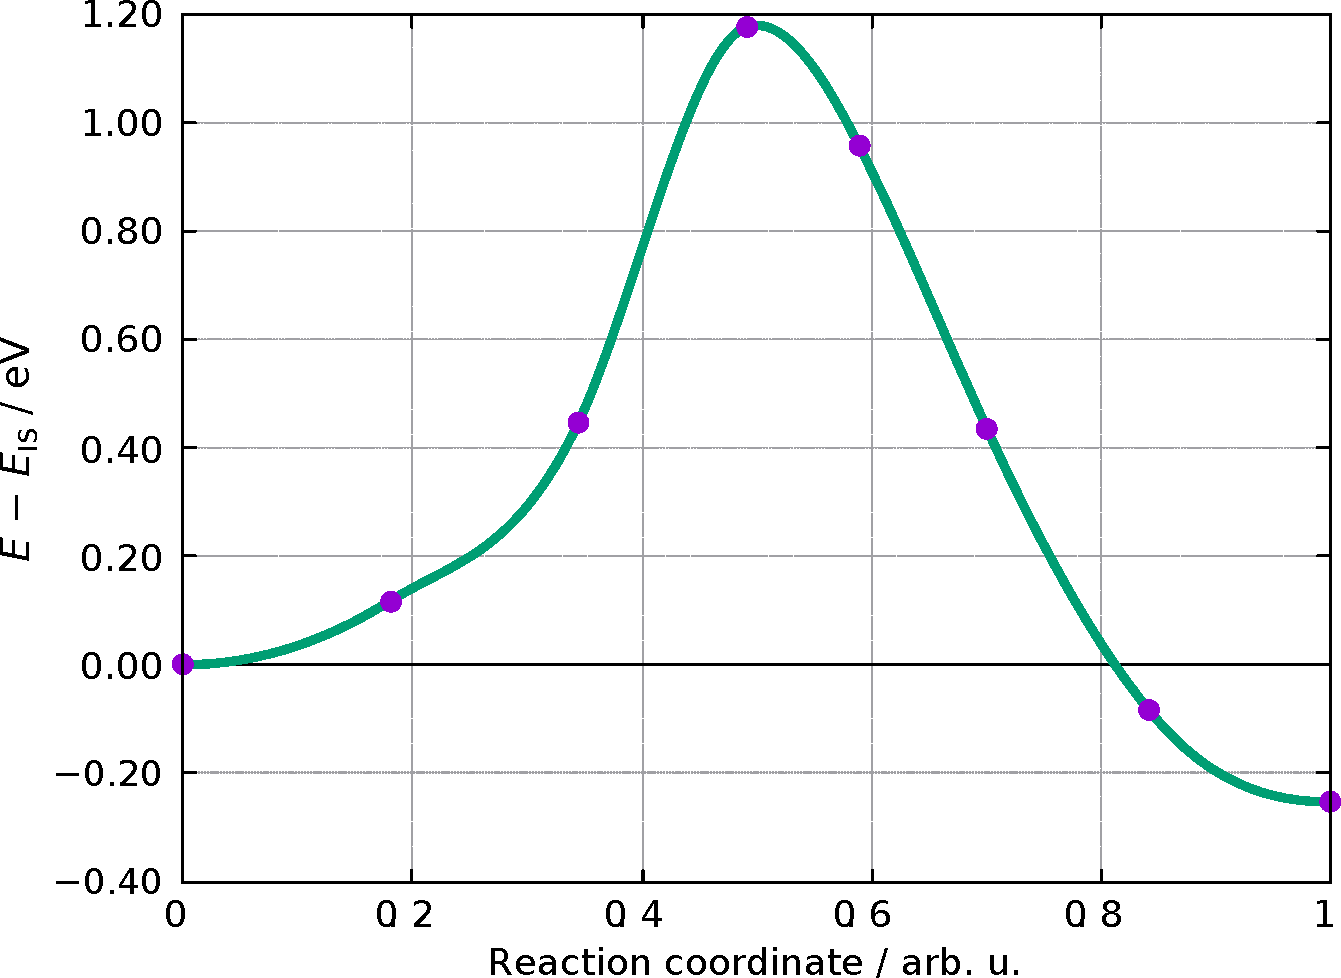
\includegraphics[width=14.cm]{figs/NEB-H2onAl100-results.pdf}
\end{figure}


%%%%%%%%%%%%%%%%%%%%%%%%%%%%%%%%%%%%%%%%%%%%%%%%%%%%%%%%%%%%% 
\head{4. PWTK: a short tutorial}
\rightheader{
\includegraphics[width=2.5cm]{figs/pwtk.png}}
\rightfooter{Example: \file{Day-3/example4.pwtk}}

PWTK is a Tcl-based scripting interface for Quantum ESPRESSO. It aims
at providing a flexible and productive framework.

\begin{itemize}
\item PWTK web-site is:\\
  \file{http://pwtk.quantum-espresso.org/} ~or~ \file{http://pwtk.ijs.si/}
\item PWTK documentation is available at:\\
  \file{http://pwtk.ijs.si/toc\_index.html}\\
  (see also \file{\href{http://pwtk.ijs.si/pwtk-slides.pdf}{http://pwtk.ijs.si/pwtk-slides.pdf}})
\end{itemize}

\begin{itemize}
\item  Move to \file{Day-3/example4.pwtk} directory. Therein are three
  examples:
  \begin{itemize}
  \item \file{ex1.eos/} -- how to use EOS (equation-of-state) utility
    of PWTK
    \vspace{0.5em}
  \item \file{ex2.O@Al111/} -- how to run many calculations with a
    simple PWTK script
    \vspace{0.5em}
  \item \file{ex3.CO@Rh100/} -- a more elaborate PWTK example that
    shows how to glue together various calculations. In particular, it
    analyzes the bonding of CO molecule on Rh(100).
  \end{itemize}
\end{itemize}

%%%%%%%%%%%%%%%%%%%%%%%%%%%%%%%%%%%%%%%%%%%%%%%%%%%%%%%%%%%%% 
\head{5. PWTK: hierarchical configuration}
\rightheader{}

\begin{itemize}
\item Main user configuration file: \file{\$HOME/.pwtk/pwtk.tcl}
  \begin{itemize}
  \item executables and how to run them (\cmd{bin\_dir}, \cmd{prefix},
    \cmd{postfix})
  \item special directories (\cmd{pseudo\_dir}, \cmd{outdir}, \cmd{wfcdir})
  \end{itemize}
\item Project-based configuration (via \cmd{import}), e.g,:  
  \begin{itemize}
  \item \file{Day-3/example4.pwtk/common.pwtk}\\[0.3em]
    Specification of default input data that are common to all examples in
    \file{example4.pwtk/}, e.g., cutoff energies, list of
    pseudopotentials, etc.
    \vspace{0.5em}
    {\small
      \begin{itemize}
      \item {\bf Beware:} for each specific calculation PWTK filters atomic
        species and uses only those that are actually used. Due to that
        the index of species can change from case to case, hence for
        {\em ntyp}-type variables do not use numeric indices, but use
        atomic labels instead, e.g.:\\
        \var{starting\_magnetization({\bf 1}) = 1.0} ~~~({\burgundy\em not recommended})\\
        \var{starting\_magnetization({\bf Fe}) = 1.0} ~~({\green\em recommended})
      \end{itemize}
    }
    \vspace{0.5em}
  \item in a given example the project-based \file{common.pwtk} is
    then imported via, e.g.,
    \file{import ../common.pwtk}
  \end{itemize}
\end{itemize}

\head{5. PWTK: concept of input data stacking}
\rightheader{}

{\small Input data stacking is a useful concept when performing
  multiple calculations. In such a case, one typically defines a set
  of default parameters for all calculations. However, each individual
  calculation may require some modification of the input data, yet it
  is inconvenient if such a change would affect the input data for
  other subsequent calculations.
  %
  This inconvenience can be prevented with \cmd{input\_push} and \cmd{input\_pop}
  commands (actually it is more convenient to use \cmd{input\_pushpop
    \{...\}} instead). The concept is illustrated below:}

\centerline{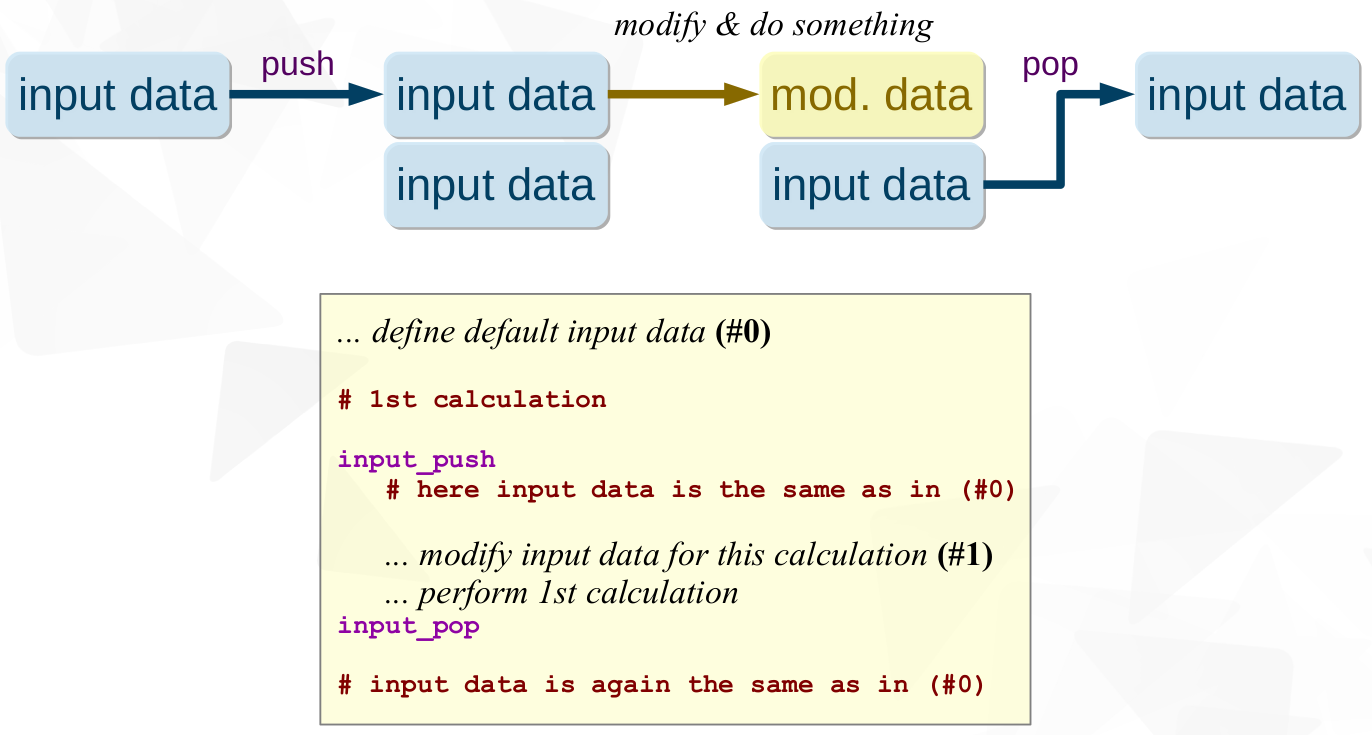
\includegraphics[width=0.8\textwidth]{figs/i-data-stacking.png}}

%%%%%%%%%%%%%%%%%%%%%%%%%%%%%%%%%%%%%%%%%%%%%%%%%%%%%%%%%%%%% 
\head{5.1 PWTK: EOS utility}
\rightfooter{Example: \file{Day-3/example4.pwtk/ex1.eos}}

Move to \file{Day-3/example4.pwtk/ex1.eos} directory.

In this example the
{\em equation-of-state (EOS)} will be calculated using
\prog{pwtk}. Run this calculation by typing:\\
\exec{pwtk eos.Rh-bulk.pwtk > eos.Rh-bulk.log \& }

This procedure performs 15 SCF calculations with different lattice
parameters (using the initial guess as input) and then uses the
results as input for \prog{ev.x}, to calculate EOS in accordance with
the four equations of state. The results are then summarized in
\file{eos.Rh-bulk.RESULTS} {\small (the \file{*.dat} data-files with
  collected total energies are contained in
  \file{eos.Rh-bulk.d/*.dat})}.

\begin{figure}
\centering
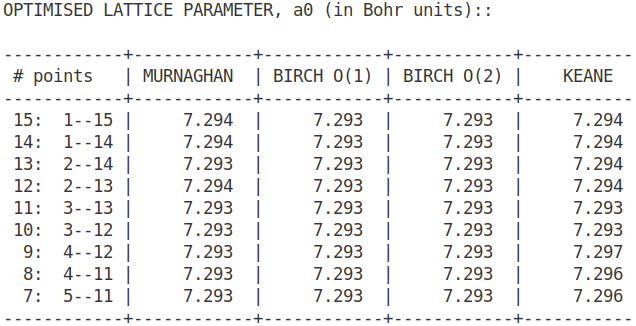
\includegraphics[width=14.0cm]{figs/LATTICE_PARAMETERS.png}
\end{figure}

Notice that the bulk-modulus is more sensitive to the sampling of
data points, can you tell why?
 
\begin{figure}
\centering
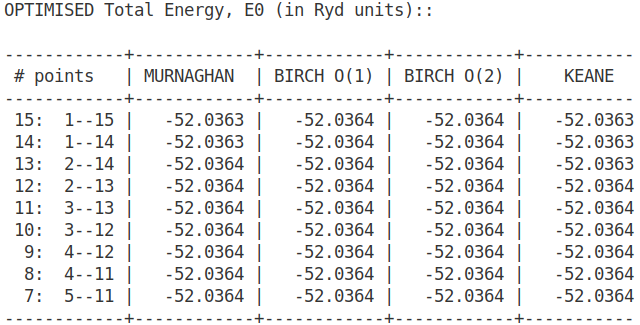
\includegraphics[width=15.0cm]{figs/TOTAL_ENERGY.png}
\end{figure}

\begin{figure}
\centering
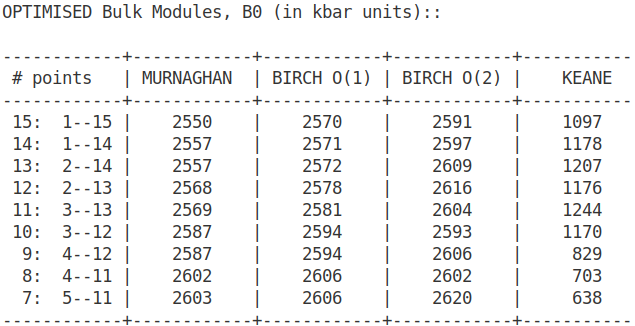
\includegraphics[width=15.0cm]{figs/BULK_MODULES.png}
\end{figure}

%%%%%%%%%%%%%%%%%%%%%%%%%%%%%%%%%%%%%%%%%%%%%%%%%%%%%%%%%%%%% 
\head{5.2 PWTK: gluing together many calculations}
\rightfooter{Example: \file{Day-3/example4.pwtk/ex2.O@Al111}}

The subject of this example is the calculation of a 2D potential
energy scan of lateral positions of O @ Al(111). It introduces the
PWTK's concept of input-data stacking (i.e. \cmd{input\_pushpop
  \{...\}}).

The corresponding PWTK snippet is:
{\codecolor\small
\begin{verbatim}
foreach ia [seq 0.0 0.2 1.0] {
   foreach ib [seq 0.0 0.2 1.0] {

      set x [expr $ia - 0.5*$ib]
      set y [expr sqrt(3)/2*$ib]

      input_pushpop {
         insertAtoms begin "O  $x $y 1.35   0 0 1"
         runPW pw.O-Al111.$ia.$ib.in
      }
   }
}
\end{verbatim}
}

Beware that without the use of input-data stacking, each new iteration
would add a new O atom to the structure. But with \cmd{input\_pushpop
  \{...\}}, we add an O atom, make a calculation, and pop the O atom
away.

The full script is provided by \file{scan.pwtk}; read it and and try
to understand it.

{\bf Beware:} this example takes quite long! Hence, it is better to
submit it to HPC cluster. This can be achieved by:\\[0.5em]
\exec{remote\_pwtk scan.pwtk}\\[0.5em]
After calculation finishes, download the output and data files as:\\[0.5em]
\exec{rsync\_from\_hpc .}\\[0.5em]
The resulting potential-energy-surface can be visualized as:\\[0.5em]
\exec{gnuplot plot2D.gp}\\[0.5em]
Then plot the result with gnuplot. You should obtain something like
this.\\

\centerline{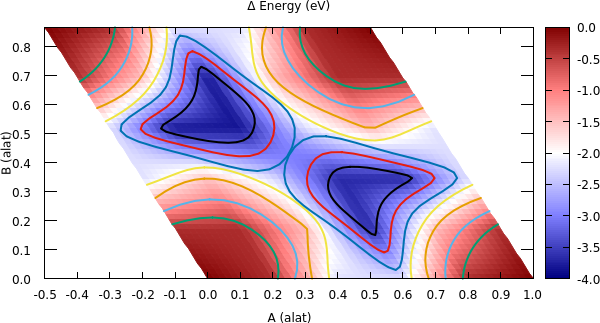
\includegraphics[width=0.475\textwidth]{figs/PES-2D.png}}


%%%%%%%%%%%%%%%%%%%%%%%%%%%%%%%%%%%%%%%%%%%%%%%%%%%%%%%%%%%%% 
\head{5.3 PWTK: analysis of electronic structure of CO@Rh(100)}
\rightfooter{Example: \file{Day-3/example4.pwtk/ex3.CO@Rh100}}

This is a bit more elaborate PWTK example that shows how to glue
together various calculations. In particular, it analyzes the bonding
of CO molecule on Rh(100) by means of (i) charge-density difference,
(ii) PDOS to atomic orbitals, (iii) MOPDOS to molecular orbitals, and
(iv) ILDOS (integrated-local density of states).

The analysis reveals the charge-donation from the CO $\sigma$ HOMO
orbital into metal states and back-donation of charge from metal
states into the CO $\pi^*$ LUMO orbital.

The master PWTK script that performs the whole analysis is
\file{run-all.pwtk}. This file imports several script, each performing
specific task(s), in particular:

\begin{itemize}
\vspace{-0.5em}
\item \file{relax.pwtk} -- script for relaxing the CO@Rh(100)
  structure
\vspace{-0.5em}
\item \file{difden.pwtk} -- script for calculating charge-density
  difference
\vspace{-0.5em}
\item \file{ildos.pwtk} -- script for calculation of ILDOSes
\vspace{-0.5em}
\item \file{pdos.pwtk} -- script for calculating PDOS to atomic
  orbitals, MOPDOS to molecular-orbitals of CO, and plots of
  molecular-orbitals ($\psi^2$) of CO (BEWARE: this is a more
  elaborate script)
\end{itemize}

%%%%%%%%%%%%%%%%%%%%%%%%%%%%%%%%%%%%%%%%%%%%%%%%%%%%%%%%%%%%% 
\head{5.3.1 DIFDEN utility}

PWTK has a {\em DIFDEN} utility to aid at calculating, e.g.,
charge-density difference:\\[0.5em]
{\black$\displaystyle\quad\quad\Delta\rho_{\rm AB}(\vr) = \rho_{\rm
    AB}(\vr) - \rho_{\rm A}(\vr) - \rho_{\rm B}(\vr)$}\\[0.5em]
({\em remark:} with {\em DIFDEN} you can calculate any difference, does not
need to be density)\\[0.5em]
%
The above difference can be calculated using the following PWTK
snippet (the CO@Rh(100) example):\\
\begin{tabular}[t]{ll}
  \begin{minipage}[t]{.4\linewidth}
\codecolor\small
\begin{verbatim}
DIFDEN {
    segment(1) = "all"
    weight(1)  = 1.0
    name(1)    = "all"
    
    segment(2) = "1 2"
    weight(2)  = -1.0
    name(2)    = "CO"
    
    segment(3) = "3-"
    weight(3)  = -1.0
    name(3)    = "Rh100"
}
difden_run difden.CO-Rh(100)
\end{verbatim}    
\end{minipage}
  &
    \begin{minipage}[t]{.5\linewidth}
      ~\\
      Note that the calculation of $\Delta\rho(\vr)$ requires 6 or 7
      calculations, i.e., \prog{pw.x} and \prog{pp.x} calculations
      for each of AB, A, and B. The last (7$^{\rm th}$) \prog{pp.x}
      calculation is to subtract the calculated densities. PWTK
      manages all these 7 calculations automatically.\\

      The full PWTK script for calculating the $\Delta\rho(\vr)$ of
      CO@Rh(100) is provided by file \file{difden.pwtk}.
    \end{minipage}
\end{tabular}

%%%%%%%%%%%%%%%%%%%%%%%%%%%%%%%%%%%%%%%%%%%%%%%%%%%%%%%%%%%%% 
\head{5.3.2 ILDOS}

ILDOS = integrated local density of states:\\[0.5em]
{\black
$\displaystyle
N(E_{\rm min},E_{\rm max},\vr) = 
 \int_{E_{\rm min}}^{E_{\rm max}}  n(\epsilon,\vr) d\epsilon 
 = \sum_v\sum_{\vk}
  \int_{E_{\rm min}}^{E_{\rm max}} |\psi_{v,\vk}(\vr)|^2 \times
  \delta(\epsilon-\epsilon_{v,\vk}) d\epsilon.$
}

\begin{center}
  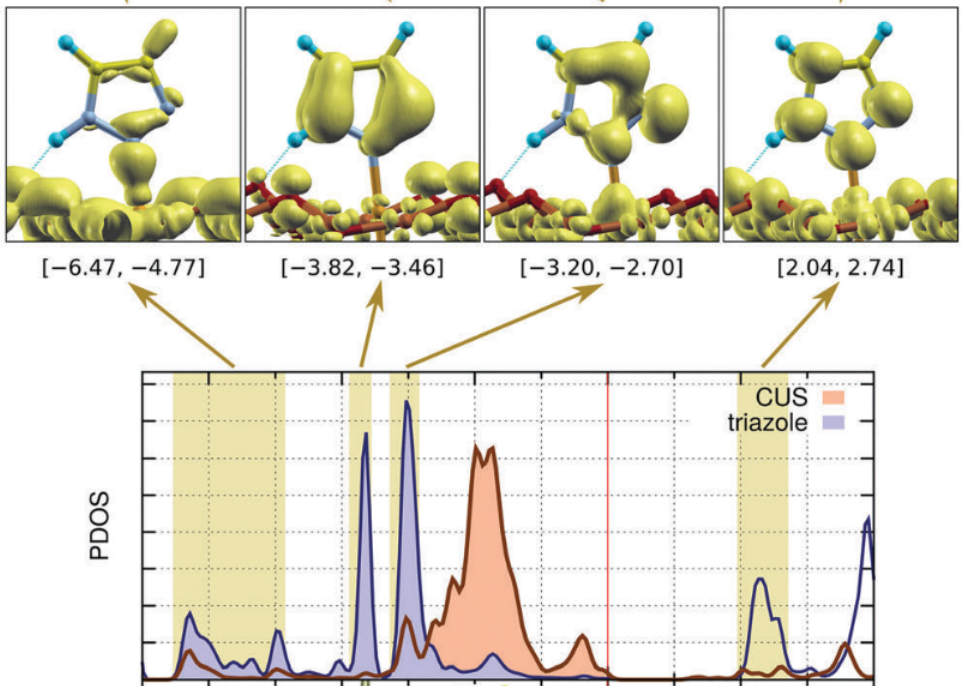
\includegraphics[width=0.6\textwidth]{figs/ildos.png}
\end{center}

%%%%%%%%%%%%%%%%%%%%%%%%%%%%%%%%%%%%%%%%%%%%%%%%%%%%%%%%%%%%% 
\head{5.3.2 ILDOS}
With aid of PWTK, a series of ILDOSes can be calculated using the following snippet:
{
  \codecolor\small
\begin{verbatim}
INPUTPP " plot_num = 10 "

foreach {Emin Emax} {
    -6.00 -5.50
    -3.40 -3.30
    -3.05 -2.95
     ...   ...
} {
    INPUTPP " emin = $Emin, emax = $Emax "
    PLOT " fileout = 'ildos.${Emin}.${Emax}.xsf' "

    runPP pp.ildos.${Emin}.${Emax}.in
}
\end{verbatim}
}

The full PWTK script for calculating a series of ILDOSes of
CO@Rh(100) is provided by file \file{ildos.pwtk}.

%%%%%%%%%%%%%%%%%%%%%%%%%%%%%%%%%%%%%%%%%%%%%%%%%%%%%%%%%%%%% 
\head{5.3.3 PDOS and MOPDOS}

The PWTK script \file{pdos.pwtk} is a bit more lengthy/elaborate. It
calculates PDOS (projected-density-of-states) to atomic orbitals,
MOPDOS (molecular-orbital projected-density-of-states) to
molecular-orbitals of CO, and it plots molecular-orbitals
($\sign(\psi(\vr))\psi^2(\vr)$) of CO.

For further details, see \file{README.md} and the \file{pdos.pwtk}
script itself. The purpose of this script is to demonstrate a bit more
advanced usage of PWTK to those who may be interested.


\end{document}

%%% Local Variables:
%%% mode: latex
%%% TeX-master: t
%%% End:
